\documentclass[12pt]{article}
\usepackage[utf8]{inputenc}
\usepackage{amsmath}
\usepackage{amssymb}
\usepackage{graphics}
\usepackage{graphicx}
\usepackage{array}
\usepackage{hyperref}
\usepackage{xcolor}
\usepackage{float}
\usepackage[french]{babel}
\usepackage[T1]{fontenc}
\usepackage[a4paper, total={6.5in, 10in}]{geometry}

\begin{document}
\begin{titlepage}
	\centering
	
	
	\vspace{0.5cm}
	{\Large \scshape\bfseries KT IT responsible}
	\vspace{0.5cm}

	{ \Huge }
	

	{\itshape V2023.1 \large  Jacques HOGGE \par}
	{\itshape V2023.2 \large  Jacques HOGGE \par}
	{\itshape V2024.1 \large  Guillaume Dupont \par}

	\vspace{5cm}
	
	
	\textit{Il s'agit d'une reformulation du KT d'avant car on a du changer de site et donc tous n'est plus trop a jour (bis)}
	

	\vfill
	
    {\Large  \today}
\end{titlepage}
\newpage

\section{GoogleSites}\label{GoogleSites}
	Notre site est géré et hébergé par GoogleSites et nous avons les noms de domaines avec OVH.
	
	\subsection{Accès au site}
		Pour accéder au site, tu dois juste te rendre sur le drive de l'addresse mail IT. Dans ce drive se trouve le site et tous les documents (images, pdf, ...) qui se trouvent sur le site.
	 	\begin{figure}[htp]
			\centering
			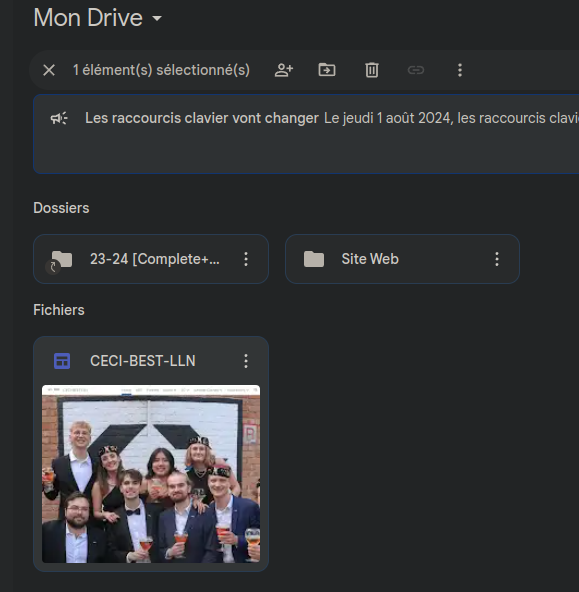
\includegraphics[width=0.6\textwidth]{img/AccessSite.png}
		\end{figure} 

	 \subsection{Évènements}
	 	Il faudra a certain moment crée une nouvelle page afin de parler d'un évènement que l'on organise (EC (RIP EBEC), Hackathon, Summer ...). Normalement c'est les MO (ou responsable du poste) de l'event qui est responsable de rédiger l'article a mettre sur la page.Il faut donc pas hésiter a les SPAM comme des porc afin d'avoir l'article a temps. Je vous conseille de poser un DL sinon il ne va jamais vous faire ton article car il est "occupé a autre chose".
	 	
	 	Bien que il y a Facebook, Insta, Onlyfans pour faire la pub de nos events et que le site est un peu obsolète, celui-ci sert principalement d'archive de CECI-BEST. Il faut cependant quand meme faire l'article car celui-ci permet un visuel pour nos sponsors.
	 	
	 	Pour faire une page, il suffit de copier une page déja faite et changer le titre, les photos, le texte, les responsable et ajouter des boutons qui ramène vers le formulaire d'inscription et/ou a l'event Facebook.
	\newpage
	 \subsection{Créer une page}
	 	Rien de très sorcier, il suffit d'aller en bas à droite sur le petit menu +.
	 	\begin{figure}[htp]
			\centering
			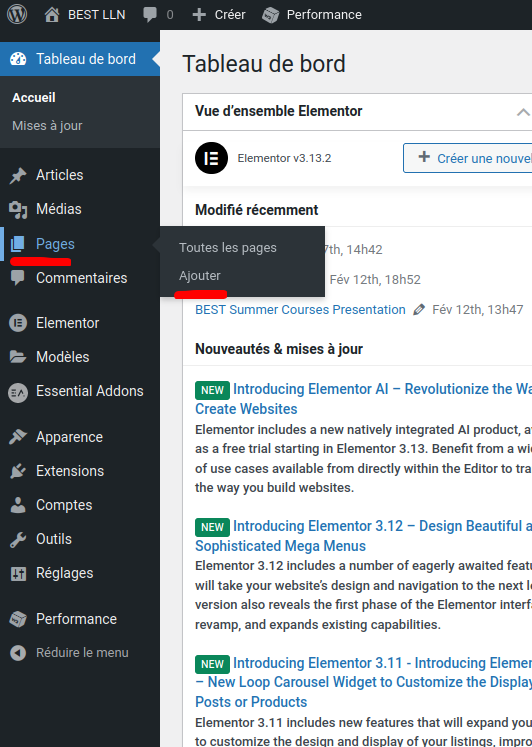
\includegraphics[width=0.6\textwidth]{img/CreerPage.png}
		\end{figure}
		
		Pour garder de jolies URL, il faut masquer la page de la navigation.
		\begin{figure}[htp]
			\centering
			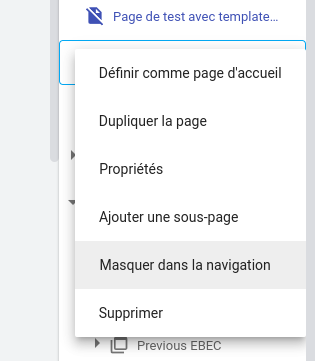
\includegraphics[width=0.6\textwidth]{img/Mask.png}
		\end{figure}

		Ensuite tu cliques sur la section où tu veux mettre la page et tu vas rajouter un lien comme si tu faisais une nouvelle page.

		Pour remplir la page inspire toi des précédents articles pour garder une certaine cohérence sur le site.
		
	\subsection{Editer une page}
		Encore moins compliqué qu'en créer une. Tu cliques juste sur la page que tu veux modifier et puis tu veux ce que tu veux.
		
	\subsection{Sponsors}
			
	Il est obligatoire de tenir notre pages des sponsors a jour, c'est dans le contrat que on leur donneras de la visibilité donc si on le fait pas on est dans la merde.
	Pour se faire, il suffit de demander au FR quelle sponsors doivent etres mis sur le site et avec quelle photo et texte. Il ne faut pas hesiter a obliger les photos et le texte au FR car peut etre que les entreprises on des exigences particulière. Ou alors vous pouvez aller voire dans le drive du FR, si celui-ci est doué, tous est la.
	Attention certain sponsors sont a l'année alors que d'autre sont peut etre juste pour un événement, a toi de demander et savoir mettre en jour en fonction de cela. 
	Tu peux juste dupliquer une des précédentes sections et changer avec la photo et le texte que tu as reçu.	
	En plus de la page sponsors, il faut aussi les ajouter sur la page  de l'event et sur la page d'accueil.Pour la page d'accueil tu peux le mettre dans le peit carousel avec les autres sponsors et pour l'event, tu rajoutes une petite photo. Dans les deux cas mets un petit lien qui redirige vers la page des sponsors.
	
	\subsection{Nouveaux et Anciens Board}
	Une fois les photos de l'ouverture reçues, tu peux mettre à jour la page du Board actuel avec la photo de groupe et individuelles.
	Plus un blague que un point réel mais les anciens veulent le moment de gloire et oblige que ils soient présent sur la page des anciens Board avec l'année du board et le Nom de celui-ci avec chaque photo et leur poste.
	Pour t'aider j'ai créer une page template dont tu peux copier la section pour remplir sur la page avec les anciens Board.
	\begin{figure}[htp]
		\centering
		
\includegraphics[width=0.6\textwidth]{img/TemplateBoard.png}
	\end{figure} 
	
\newpage
\section{OVH}
	Maintenant OVH nous sert que pour nos noms de domaine: \textit{www.best-lln.eu} et \textit{www.best-lln.be}\footnote{C'est le nom de domaine de l'ancien site, on a garder le nom de domaine et fait une redirection vers le nouveau site, ça coute pas trop cher donc a voir avec la trésorerie si vous le laisser ou pas}. 
	
	\subsection{Noms de domaines}
	Comme dis juste au dessus, on a deux noms de domaines. La seule chose que tu as à faire, c'est de pas oublier de les renouveler. Oublie pas de metrte des rappels ou autres, ça tombe juste après les examens donc oublie pas. Pour payer le renouvelement, idéalement, demande la carte de banque CECI, mais si c'est pas possible et qu'il reste pas beaucoup de temps, paaies toi-même et envoies les détails au trésorier.
	\begin{figure}[htp]
		\centering
		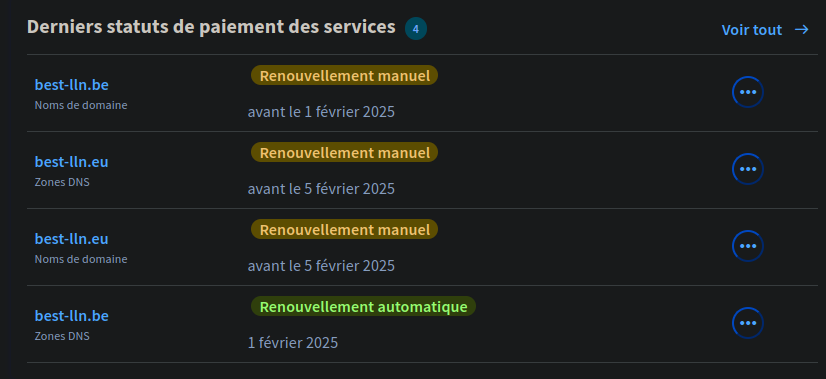
\includegraphics[width=0.6\textwidth]{img/NomsDomaine.png}
	\end{figure}

	\subsection{Redirection}
		Avant on passait par le menu \textit{Redirection} mais maintenant ça ne fonctionne plus qu'on est pas vraiment hégergé chez eux.
		\begin{figure}[htp]
			\centering
			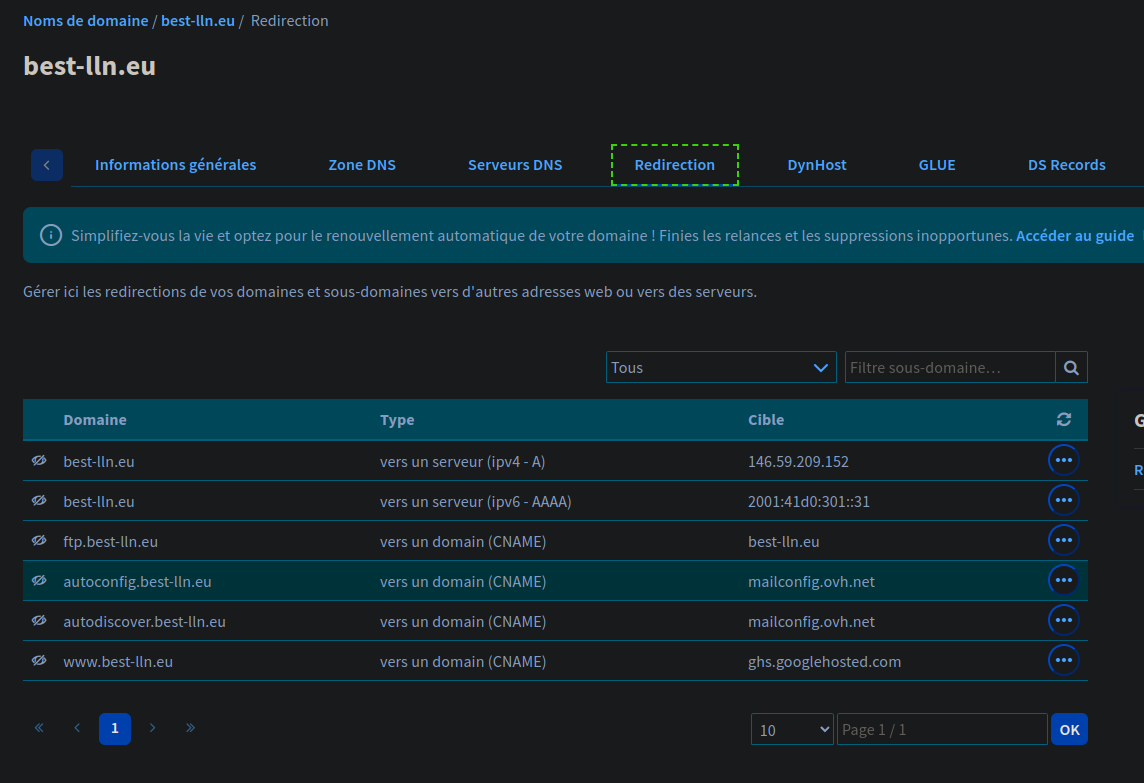
\includegraphics[width=0.5\textwidth]{img/OVH-Redirect.png}
		\end{figure}
\newpage
		On passe donc maintenant par un petit fichier sur l'hébergement gratuit associer au nom de domaine. Pour ça tu sur l'hébergement associé à \textit{www.best-lln.eu} $\Rightarrow$ \textit{FTP - SSH} $\Rightarrow$ \textit{FTP Explorer}
		\begin{figure}[htp]
			\centering
			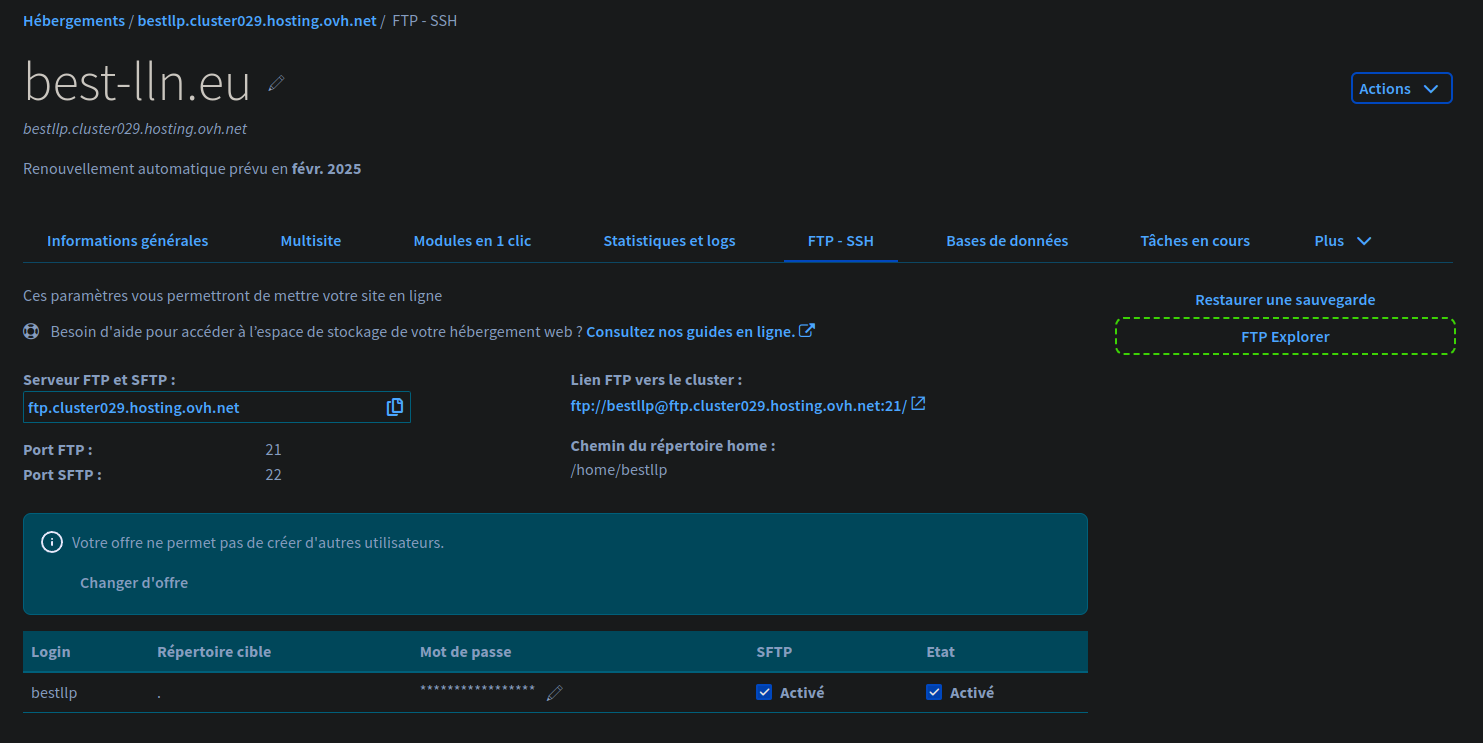
\includegraphics[width=0.6\textwidth]{img/FTP-Explorer.png}
		\end{figure}

		Il faut se connecter avec les identifiants que je te donnerais ou bien tu peux les réinitialiser. Ensuite tu vas dans le dossier \textit{www} $\Rightarrow$ \textit{.htaccess}. Et dans ce fichier, tu peux modifier les règles de redirection.
		\begin{figure}[htp]
			\centering
			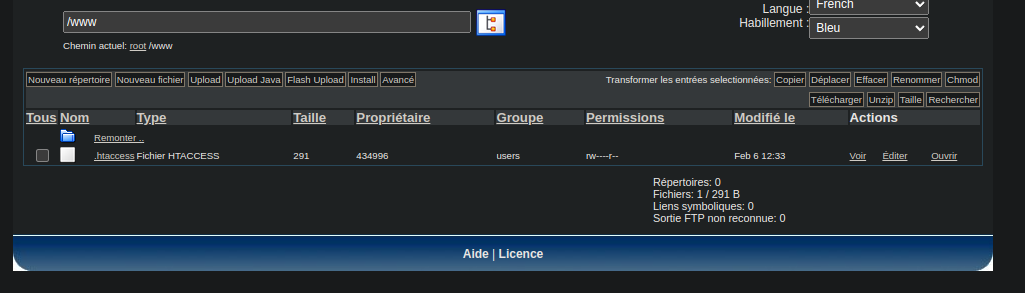
\includegraphics[width=0.6\textwidth]{img/htaccess.png}
		\end{figure}
		
	\subsection{Autre}
		Il y a plein d'autres fonctionnalités sur OVH tels que voire le trafic sur le site etc. Hésite pas a visiter et Google les ton amis et les anciens IT aussi.
		
\section{Github}
	Depuis 2023 le CECI-BEST possède une Github qui est nécessaire pour récupérer les projets des PAX des différents Hackathons. La responsabilité est techniquement celle de l'IT qui devra aller voir les différents groupes afin de s'ajouter sur le git (ou du moins de les mettre en favoris) et garder ainsi une archive. Vous pouvrez aussi les télécharger si vous avez peur qu'ils disparaîssent. 
	Sur le github, il y a moyen des créer des "dossier" qui comporte different repo github. il suffit d'en créer un par année et de rajouter les repos dedans. Cela est possible avec le syteme "favoris".
	Google est ton amis et regarde comment c'est fait avant.
	
\section{Transfert des différents comptes/identifiants}
	Pour tous les identifiants demande à l'ancien IT.
	\subsection{Addresse mail}
		C'est un peu le plus important car c'est sur le drive de ce mail que se trouve le site. Tu en auras aussi besoin pour les autres comptes et tu peux l'utiliser si tu as besoin de créer un compte sur un autre site.
	\subsection{OVH}
		\begin{enumerate}
			\item Compte OVH: Le principal pour gérer les noms de domaines et redirections.
			\item FTP Explorer: Tu as besoin d'identifiants pour pouvoir se connecter à l'hébergement pour les redirections.
		\end{enumerate}

	\subsection{Github}
		Pour Github, tu peux toujours rajouter ton mail perso en address secondaire.\footnote{Ne pas mettre la mailing list du board en addresse sinon tout le monde reçoit tous les mails. Tout le monde se plaindra, c'est du vécu.}
	
\section{Hacked}	
	Il est déja arrivé plusieur fois que on se soit fait Hacker. On parle plus d'un malware qui redirige notre site vers un site de scam. Souvent c'est parceque une script Js a été ajouté dans le header, il font donc le retrouver et le retirer.

	Normalement ça ne devrait plus arriver vu qu'on est chez Google maintenant.
	
	Assez basique mais vérifie aussi de temps-en-temps s'il n'y a pas de connexions louches, si c'est le cas, changer tous de suite les mots-de-passe. N'hésite pas à ajouter aussi une authentification a double facteur.
	
\section{Pour le futur}
	Notre site est donc sous GoogleSites mais tu le remarqueras très vite que tu es assez limité dans la création. C'est suffisant pour le minimun requis pour notre site mais si tu veux plus de personalisation et/ou ajouter d'autres choses sur le site, il faudra surêment passer par une autre solution mais ça je te laisse y réfléchir.

\section{Poste}

	IT est un poste qui selon certaines personnes ne sert a rien ou ne travaille pas. Peut importe ce que tu dit il diront que tu ne fais rien et cela est normal car ce que tu fais n'est pas directement visible.
	Donc faut pas le prendre mal quand ils disent que tu ne fais rien.
	\subsection{Slides}	
	L'IT est aussi responsable du rétroprojecteur qui est au local et qu'il faut prendre pour afficher les slides aux réunions s'il n'y pas d'écran dans la salle. Rien de très sorcier il suffit de demander au gens d'aller dans ton dossier IT sur le drive et de remplir les slides, hésite pas à créer les slides dès qu'on reçoit l'ODJ \footnote{ça paraît tout con mais certain sont très vites perdus si les slides sont pas créées à l'avance}.
	
	\subsection{Wooclap}
		Il y a deux moments où tu en auras besoin:
		\begin{enumerate}
			\item Réunions classiques: quand on élit une core team pour un event (Hackathon ou EC).
			\item LGA: là il en faut pas mal (memberships, proposals, ...).
		\end{enumerate}
		Dans les deux cas, il faut que tu les prépare à l'avance. Quand tu en as beaucoup à faire, tu peux passer par un excel, tu écris une question puis tu l'export en excel tu peux rapidement enchainer les questions.
		Pour savoir quoi mettre et les modalités de vote, il y a un document \textit{Méthode de vote pour les nuls} sur le drive (dans le dossier IT).
		Pour le compte Wooclap, utilise ton addresse UCL comme ça tu n'as pas de limites.
		
	\subsection{Clown}
		L'IT est la personne la plus drôle du Board, c'est comme ça c'est la règles, il faut donc tous le temps dires des blagues et faire des bullshit marrants. Attention il faut savoir etre sérieux quand il le faut.
	
	\subsection{\textcolor{red}{TRITOUFS}}
		
		La tradition veut que les IT soient des gens expérimentés dans l’art de BWAR. il faut donc se spécialiser dans l’art du Tritouf au fil de ton mandat, c’est pourquoi c’est un plus pour ton poste si tu sais bien en faire (ça va chier au rachat). 
		
		\begin{enumerate}
			\item Se munir de trois gobelets (réutilisables \#GreenTeam) 
			\item Les remplir généreusement avec de la bière
			\item Les aligner selon ta bonne guise 
			\item Souffler un bon coup 
			\item Boire le premier 
			\item Boire le deuxieme
			\item Boire le troisieme
			\item Éventuellement vomir
			\item Recommencer à partir du point 1. 

		\end{enumerate}
		
		Le but étant bien sûr de vider tous ses verres ENTIÈREMENT. Pas nécessairement le plus vite possible MAIS c’est un plus, naturellement.   


		De nombreuses séances d'apprentissage seront organisées pendant le Summer Course ainsi que des séances d’examen. Bonne chance. 

\section{Conclusion}
	Le post IT c'est le meilleur
		
		
\end{document}